Each player plays when it is its turn.

\section{UML}

Here is the global UML diagram of the program:

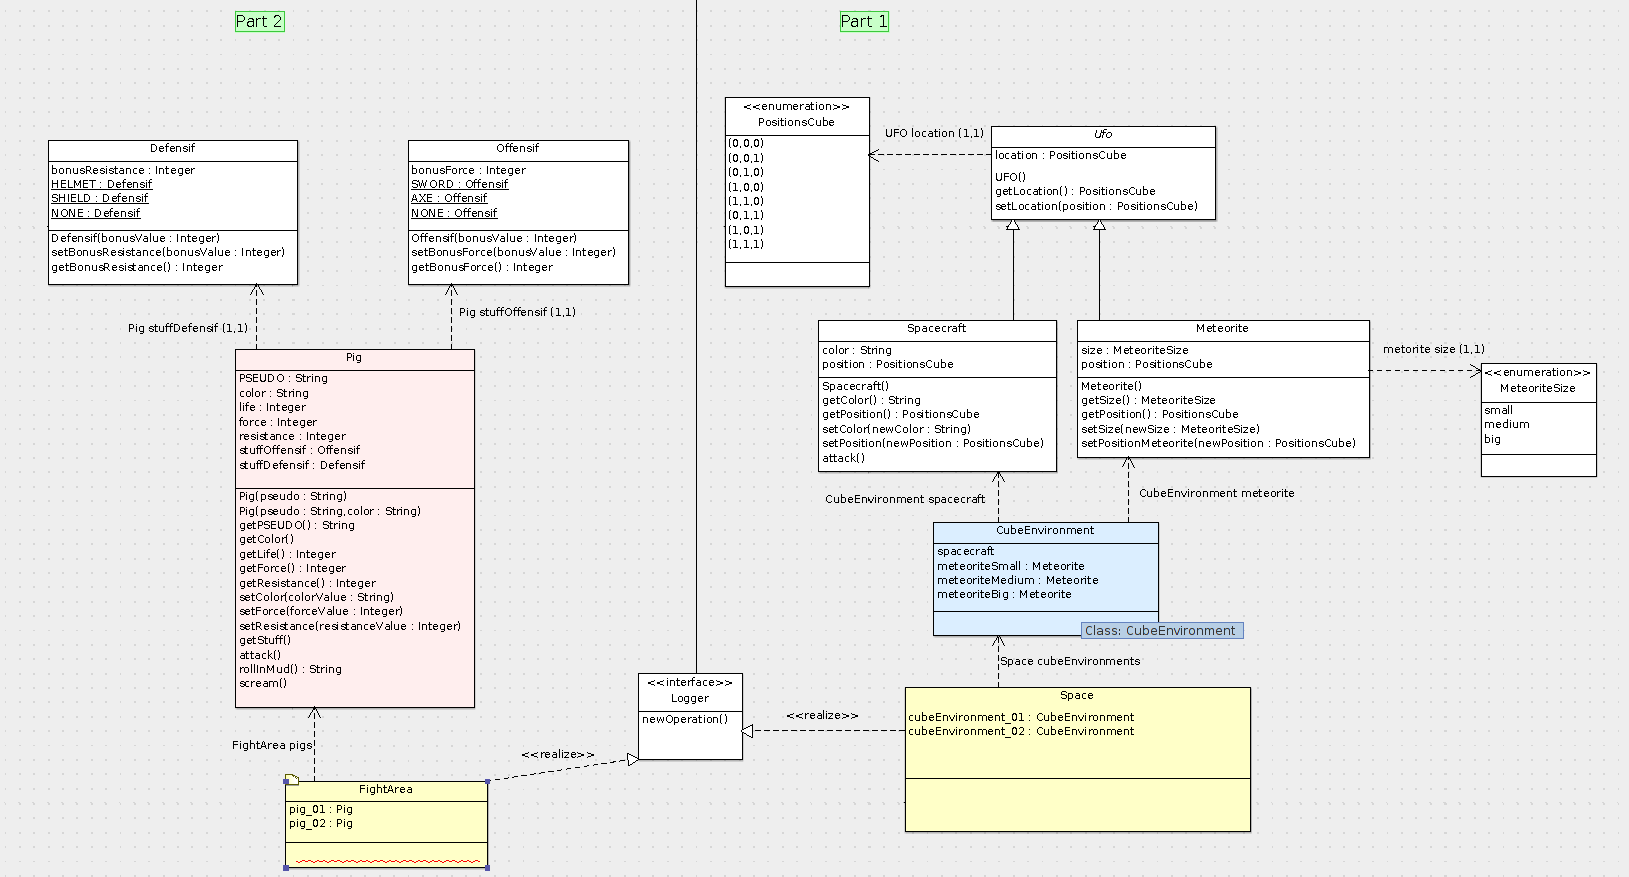
\includegraphics[width=450pt]{../../Images/UMLdiagramme.png}

Since you can't see anything on this screenshot, there bigger screenshots below.

Blue classes are abstract classes.\\
Green classes are interface.\\
Pink classes are enumeration.\\
Yellow classes are the two main classes from the 2 different parts of the game.\\

\begin{figure}
  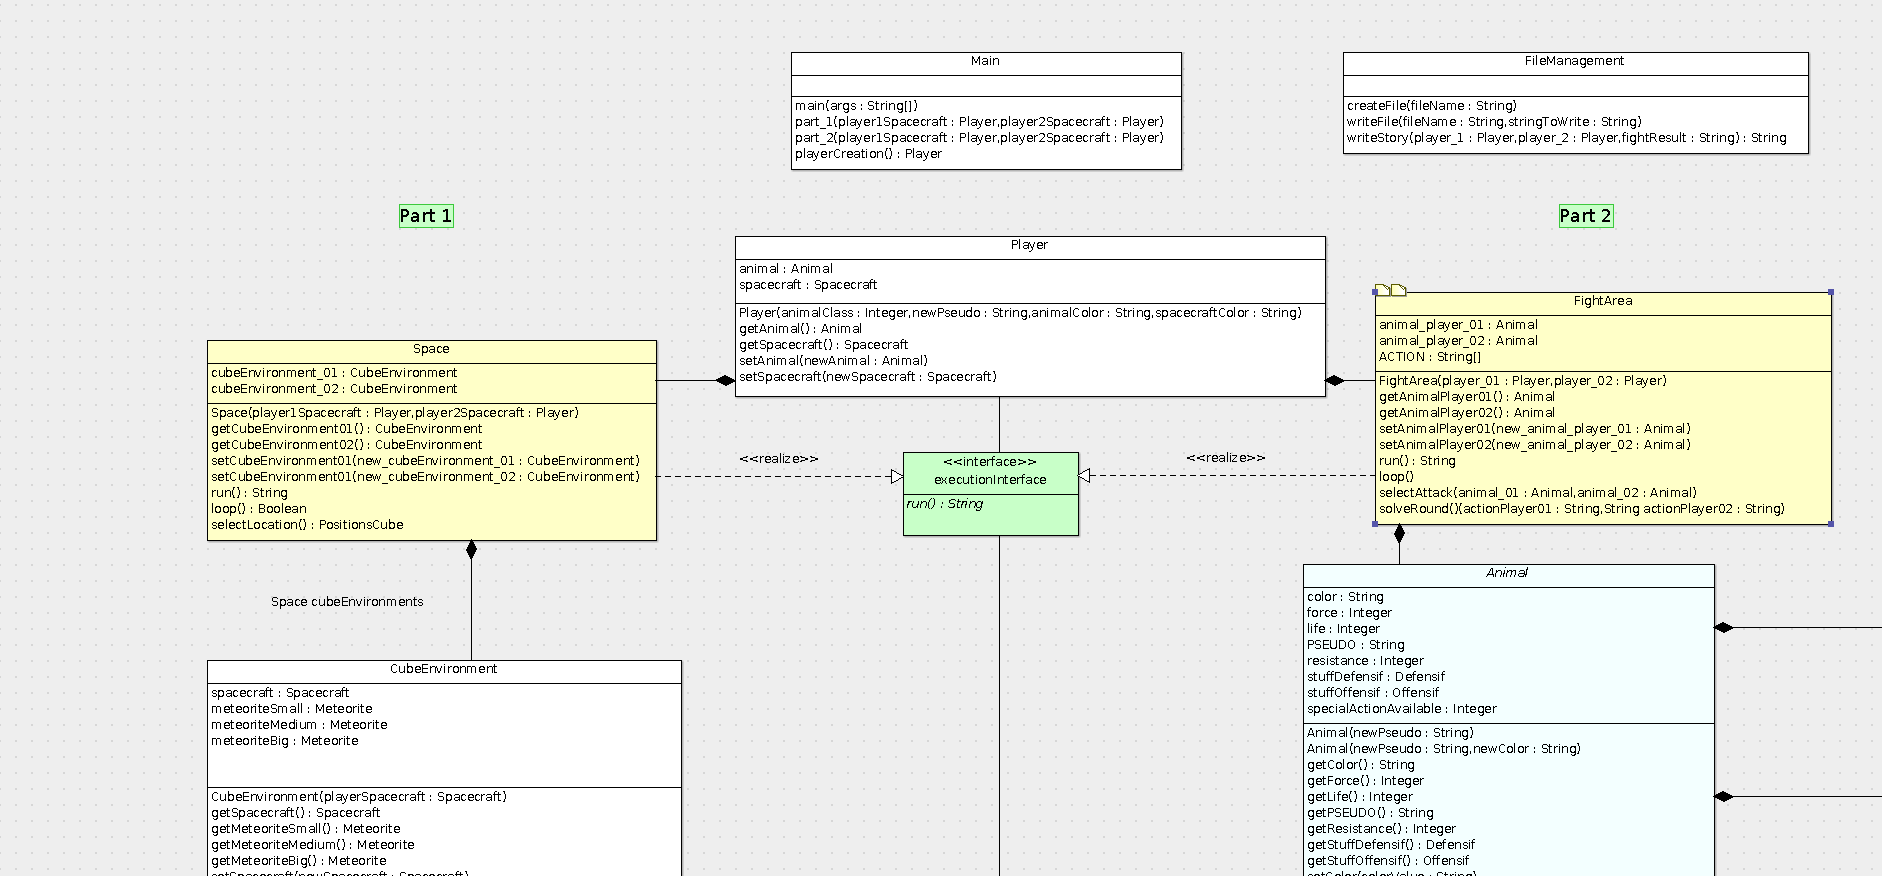
\includegraphics[width=450pt]{../../Images/1_1-2_1.png}
  \caption{\small left screenshot 1}
  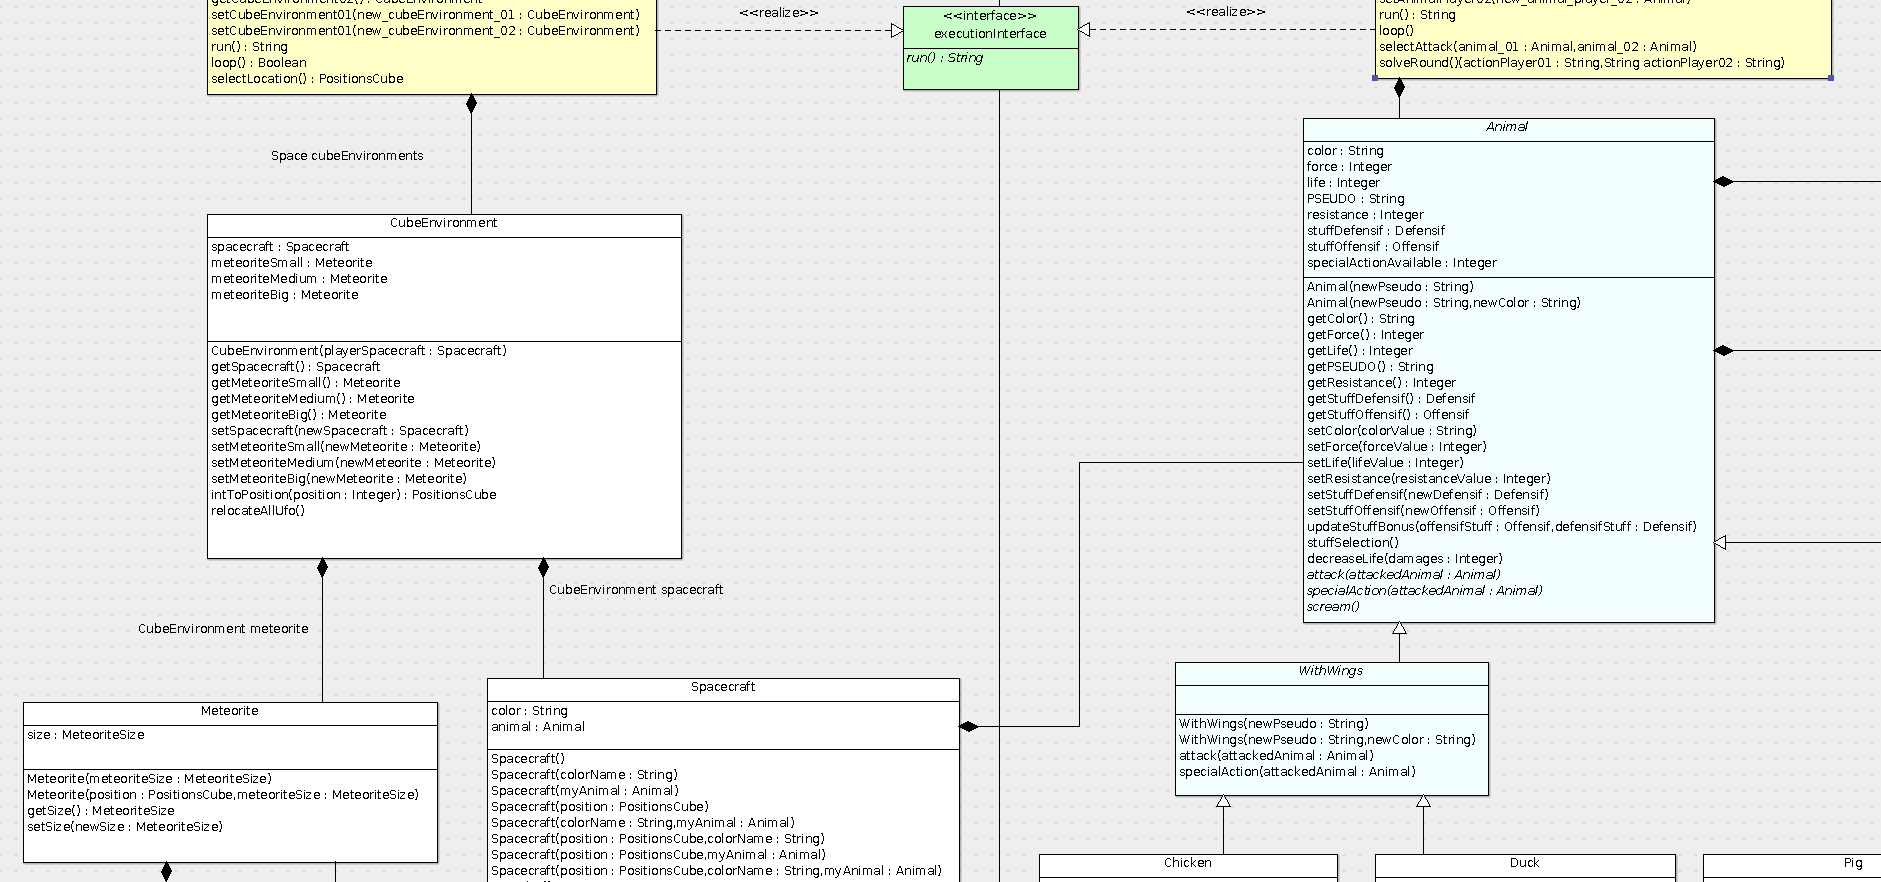
\includegraphics[width=450pt]{../../Images/1_1-1_2-2_2.png}
  \caption{\small left screenshot 2}
  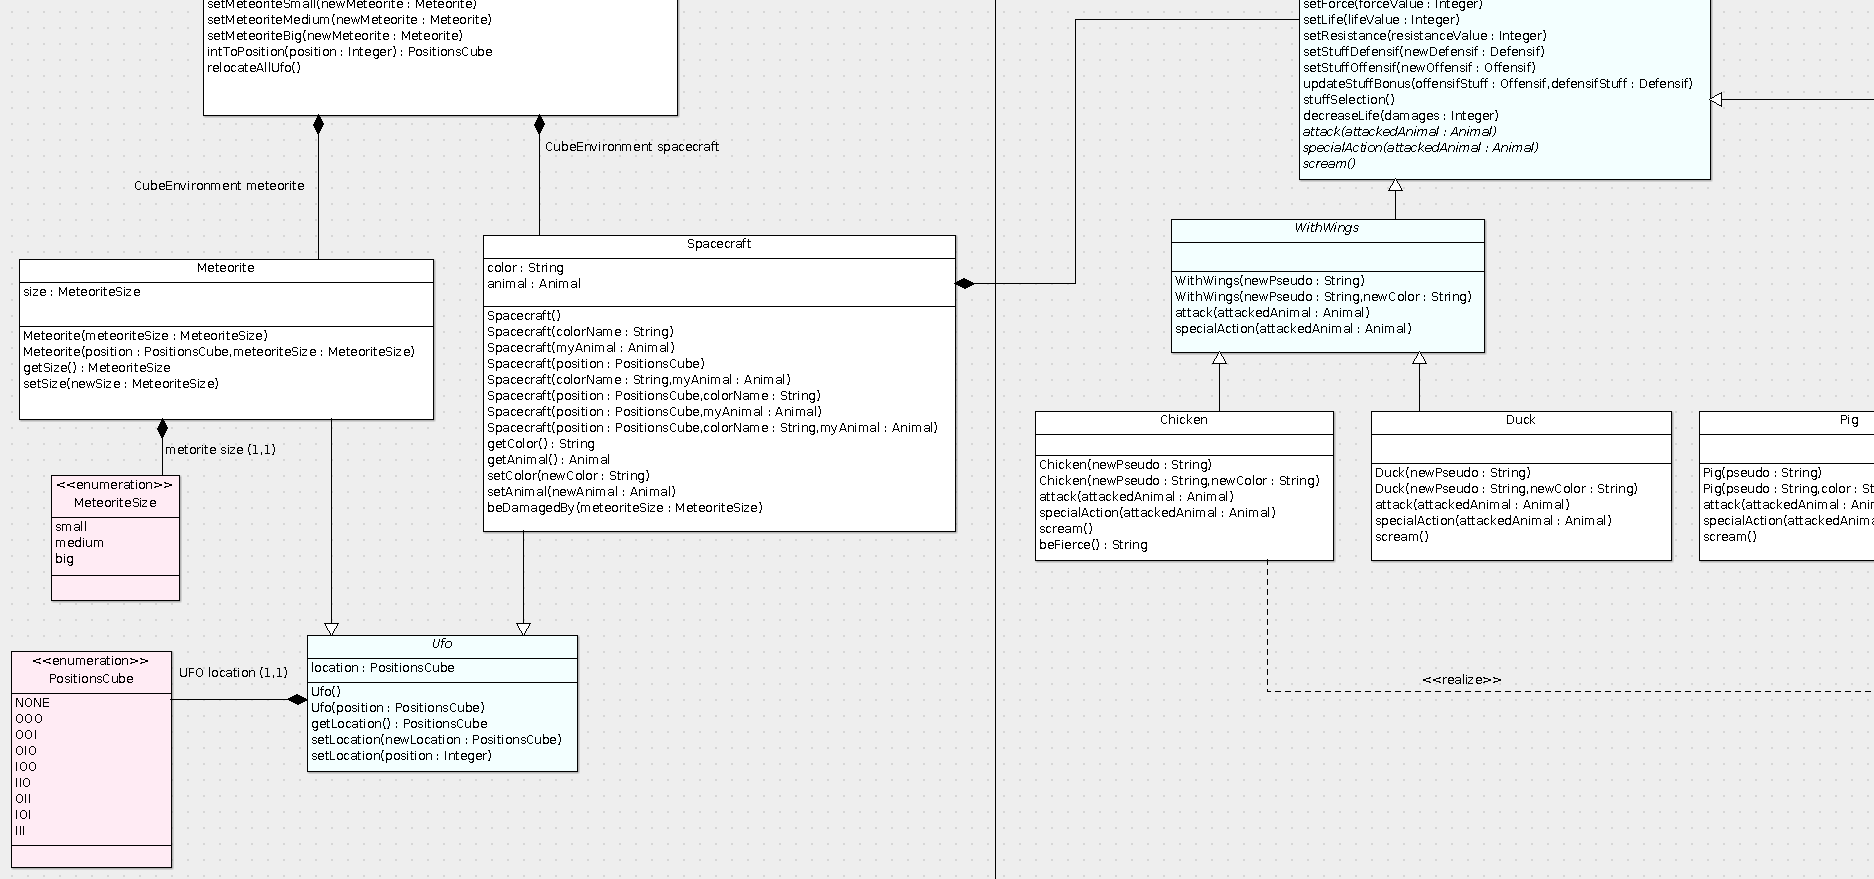
\includegraphics[width=450pt]{../../Images/1_2-2_3.png}
  \caption{\small left screenshot 3}
\end{figure}

\begin{figure}
  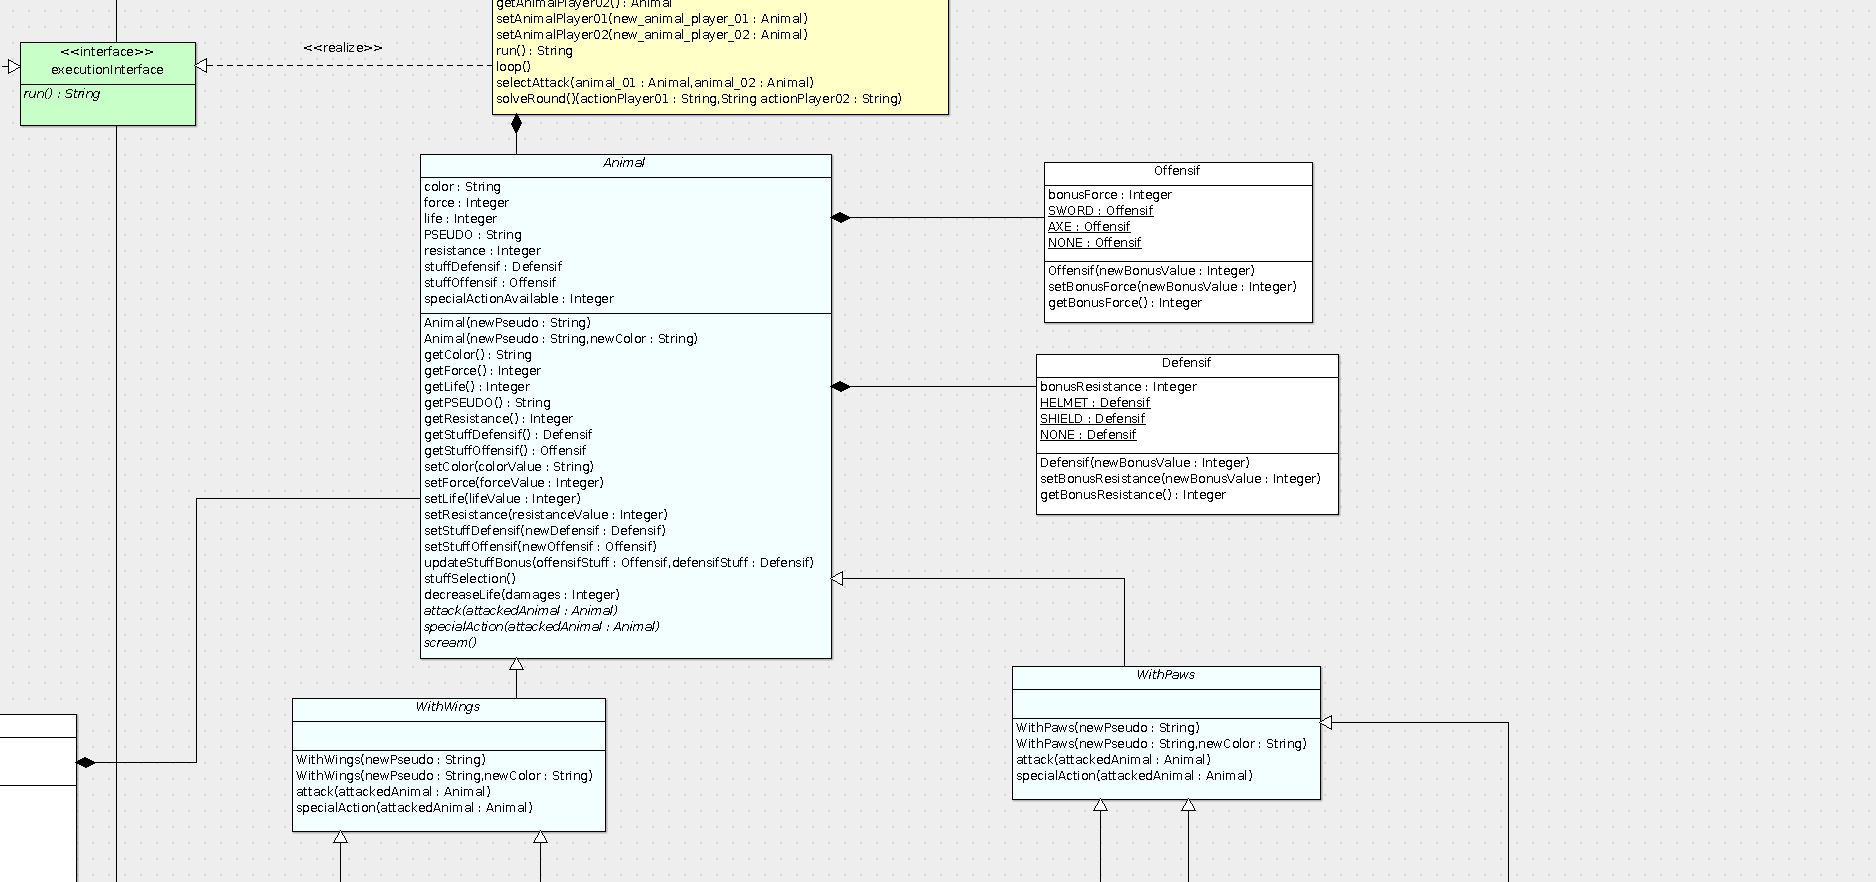
\includegraphics[width=450pt]{../../Images/2_2-3_2-3_3.png}
  \caption{\small right screenshot 1}
  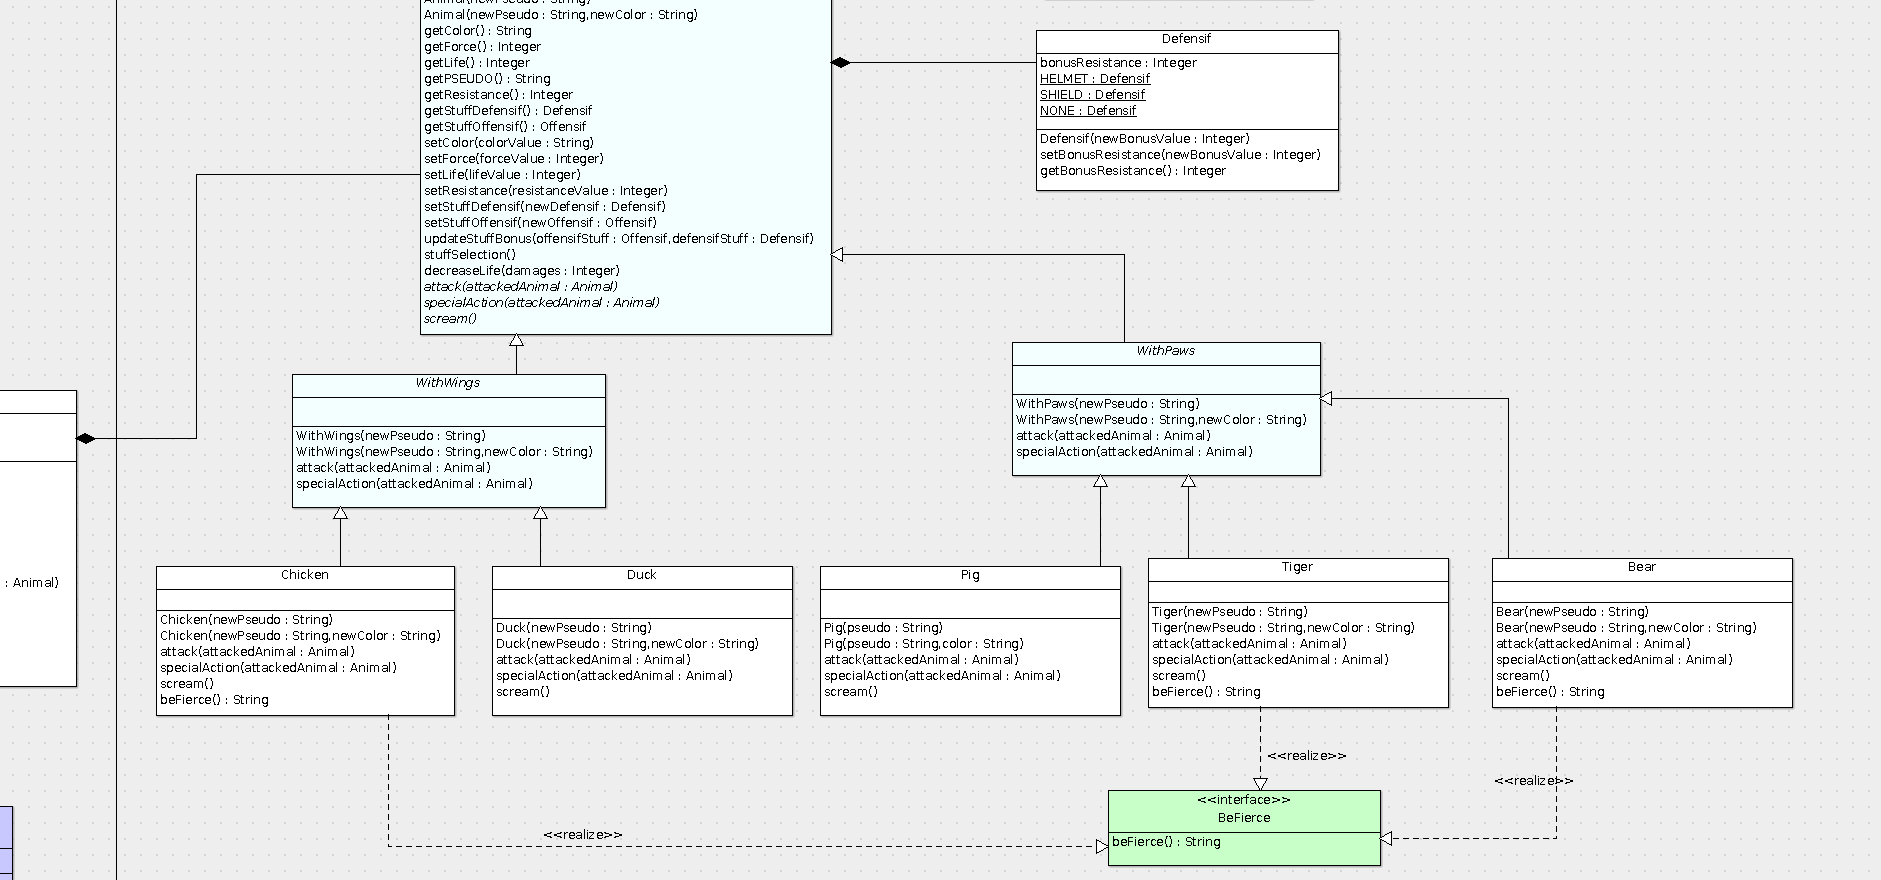
\includegraphics[width=450pt]{../../Images/2_3-3_3.png}
  \caption{\small right screenshot 2}
\end{figure}

\section{Technical part: class description}

<insert here: brief class description>

\subsection{Main}

This class contains the main functions:

\begin{itemize}
 \item main : main function that calls all the following functions.
 \item playerCreation : function that create the 2 players.
 \item part\_1 : function that runs game part 1.
 \item part\_2 : function that runs game part 2.
\end{itemize}


\subsection{FileManagement}

This class contains all useful functions to save the game story in a file.

\subsection{Player}

We created a Player class that keeps all information about each player.

\subsection{Set the game}

\begin{itemize}
 \item set Player class for each player.
 \item set Space class with 2 CubeEnvironment (1 for each player). Each CubeEnvironment is set with 3 meteorites and 1 spacecraft.
 \item set FightArea class with 2 pigs. Each pig is initialized with stuff selected by the player.
\end{itemize}


\subsection{The Space :}

It is composed by 2 CubeEnvironments created thanks to the 2 Players.

\subsection{The FightArea :}

It is composed by 2 Animals created thanks to the 2 Players.


\section{Encountered difficulties}

\subsection{Special action}

Special actions are very different. So we had to think our code so that it would be able to welcome each special action.
(We may had to modify our code ?)

\subsection{Exception}

We created an exception.


